\documentclass[a4paper,10pt]{article}
%Use article for short documents
\usepackage[T1]{fontenc}
\usepackage{parskip}
\usepackage{latexsym,amsmath,amssymb, tabu}
\usepackage[natbibapa]{apacite}
\usepackage{graphicx}
\usepackage{times}
%\usepackage{zi4}
\usepackage[a4paper,left=3cm,right=3cm,top=3cm,bottom=3cm]{geometry}
\usepackage{caption}
\usepackage{subcaption}
\usepackage[section]{placeins}
\usepackage{listings}
\usepackage[usenames, dvipsnames]{color}
\usepackage{bm}
\usepackage[retainorgcmds]{IEEEtrantools}
\usepackage{setspace}
\usepackage{multirow}
\usepackage{longtable}
\usepackage{subcaption}
\usepackage[stable]{footmisc}
\usepackage[showonlyrefs]{mathtools}
\usepackage{hyperref}
\usepackage{algorithm}
\usepackage{algorithmic}
% \usepackage[noend]{algpseudocode}

\DeclareMathOperator{\expectation}{E}

\newcommand{\euler}{\mathrm{e}}
\newcommand{\diff}{\mathrm{d}}
\newcommand{\T}{^\textup{T}}
\newcommand{\vect}[1]{\mathbf{#1}}
\newcommand{\vectGreek}[1]{\boldsymbol{#1}}
\newcommand{\matr}[1]{\mathsf{#1}}
\newcommand{\dotdotdot}{\vphantom{.}_{\cdots}}


\bibliographystyle{apacite}

\title{Learning our ABCs}
\author{Nathan Cunningham \and Sherman Ip \and Ella Kaye}

\begin{document}
\maketitle

\section{Introduction}
Approximate Bayesian computation (ABC) is a powerful tool that approximates sampling from a posterior distribution when the likelihood is intractable. ABC has found wide application in fields such as population genetics, where it is possible to simulate from models, but it is impossible, or computationally too expensive, to calculate the likelihood of the data.

In this report, we examine an implementation of ABC on 

\section{Background}
\label{sec:bg}
In a standard Bayesian inference, we wish to simulate from the posterior distribution

\[
\pi(\theta | y_\textrm{obs}) = \frac{p(y_\textrm{obs} | \theta) \pi(\theta)}{p(y_\textrm{obs})},
\]
where $y_\textrm{obs}$ are our observed data and $\theta$ a vector of parameters. However, doing so is impossible when the likelihood is intractable. By accepting some approximations, it is still possible to perform Bayesian inference in such a setting. First, the full Bayesian posterior is approximated by a partial posterior distribution

\[
\pi(\theta | s_\textrm{obs}) = \frac{p(s_\textrm{obs} | \theta) \pi(\theta)}{p(s_\textrm{obs})},
\]
where $s_\textrm{obs} = S(y_\textrm{obs})$ is a vector of summary statistics of a lower dimenion than the data. Since $\pi(\theta | s_\textrm{obs})$ is likely to be computationally intractable when $\pi(\theta | y_\textrm{obs})$ is, a further approximation must be made. In the simplest ABC algorithm, rejection sampling, the ABC posterior distribution, $\pi_{\epsilon}(\theta | y_\textrm{obs})$, is generated by Algorithm \ref{alg:ABCrej}.

\begin{algorithm}
\caption{ABC by rejection sampling} \label{alg:ABCrej}
\begin{algorithmic}
\FOR{$i = 1,\ldots, N$}
\REPEAT
\STATE Generate $\theta'$ from the prior distribution $\pi(\cdot)$
\STATE Generate $y_i$ from the likelihood $p(\cdot | \theta')$
\UNTIL{$\rho\{S(y_i), S(y_\textrm{obs})\} \leq \epsilon$}
\STATE set $\theta_i = \theta'$
\ENDFOR
\end{algorithmic}
\end{algorithm}

The idea behind ABC in Algorithm \ref{alg:ABCrej} is that when the summary statistic $S$ is representative of the data and the tolerance $\epsilon$ is small enough, then $\pi_{\epsilon}(\theta | y_\textrm{obs}) \approx \pi(\theta | y_\textrm{obs})$.

There are three components that need tuning in Algorithm \ref{alg:ABCrej}: $S(\cdot)$ which gives the summary statistic, the distance measure $\rho$, and the tolerance $\epsilon$. Throughout this report, we take $\rho$ to be the Euclidean distance measure. 

When $\epsilon = 0$, the algorithm samples from the partial posterior. A toy example of this is discussed in Section \ref{sec:beta-bin}. However, when data are continuous, and in all real-world cases, we will have $\epsilon > 0$. Selecting $\epsilon$ is a trade-off; a small $\epsilon$ gives a closer approximation to the partial posterior, whilst at the same time increasing the compuational cost by lowering the acceptance rate. One option for tuning $\epsilon$ is through cross-validation. We take this approach in Section \ref{sec:abc}.

The selection of summary statistics is also crucial to the accuracy and efficiency of ABC. Again, there is a trade-off. With a large number of summary statistics, the error in the approximation of $p(\theta | y_\textrm{obs})$ by $p(\theta | s_\textrm{obs})$ is likely to be reduced, but the approximation of $p(\theta | y_\textrm{obs})$ by $p_\epsilon(\theta | y_\textrm{obs})$ is likely to be poor because of inefficiency. On the other hand, with only a few summary statistics, the second approximation should be good, but the first will be poor. We have that $\pi(\theta | s_\textrm{obs}) = \pi(\theta | y_\textrm{obs})$ if $s_\textrm{obs})$ is a sufficient statistic. However, in many applications, it will not be possible to find sufficient statistics. In early applications of ABC, summary statistics tended to be chosen in a fairly ad hoc manner. One more principled approach is that of best subset selection, which considers whether an additional summary statistic $s_k$ should be added to a model that already contains statistics $s_1, \ldots, s_{k-1}$. Even when implemented with a step-wise search algorithm, this approach becomes computationally unwieldy whenever $k$ is large. Moreover, it needs an additional tuning parameter to determine the threshold at which each statistic is either accepted or rejected. It is also possible that an accepted statistic actually biases approximation away from the true posterior.

Another approach, proposed by Fearnhead and Prangle \cite{Fearnhead2012}, is that of semi-automatic ABC as a means of methodically selecting summary statistics for inclusion in ABC. The method proceeds as follows:

\begin{itemize}
\item Run an inital run of ABC to find a posterior region of non-negligible mass
\item Simulate parameter values and resulting proposal summary statistics
\item For each parameter run a linear regression of the summary statistics on the parameter values. Use an information criterion such as BIC to determine which summary statistics can best be used to infer the parameter values
\item Run ABC using this choice of summary statistics
\end{itemize}

We consider the effectiveness of this method in Section \cite{sec:saabc}.

There are a number of improvements that can be made to Algorithm \ref{alg:ABCrej} to correct for the distance between $S(y_i)$ and $S(y_\textrm{obs})$. One, suggested by \cite{beaumont2002} uses local linear regression, so that for each simulated $z$, we set 
\[
\theta_i = m(S(y_i)) + \eta_i
\]
where $m$ is the regression function and the $\eta_i$ are centered random variables with common variance. Instead of rejecting or accepting $\theta_i$ based on the threshold $\epsilon$, each simulation $(\theta_i, S(y_i))$ is then assigned a weight $K[\rho(S(y_i), S(y_\textrm{obs}))]$, based on a statistical kernel $K$, with higher weights given for proximity to the observation. Throughout, we use the Epanechnikov kernel. 

\section{Applications}
\subsection{Beta prior, binomial likelihood} \label{sec:beta-bin}
\subsubsection{Method}
Suppose a parameter $\theta$ has a prior distribution such that
\begin{equation}
\theta\sim\textup{Beta}(1,1)
\end{equation}
and that a random variable $X$ is distributed such that
\begin{equation}
X|\theta\sim\textup{Bin}(12,\theta) \ .
\end{equation}
Then after observing $X=2$, the posterior distribution is given as
\begin{equation}
(\theta|X=2)\sim\textup{Beta}(3,11) \ .
\end{equation}
ABC was used to sample the posterior distribution where the algorithm is as followed:
\begin{itemize}
  \item Sample $\theta$ from the uniform distribution
  \item Sample $X|\theta$ from the likelihood
  \item If the sampled $X|\theta$ is equal to 2, accept $\theta$, otherwise reject.
\end{itemize}

\subsubsection{Results}
$10,000$ posterior samples were drawn from the ABC algorithm. These were compared with the true posterior distribution, as shown in Figure \ref{binomial}, using the $\chi^2$ goodness of fit test.  By repeating the experiment $50$ times, the mean and standard deviation $p$-value for the $\chi^2$ test was found to be $(50\pm30)\%$. This was very strong evidence that the ABC posterior samples did estimate the posterior distribution well.

The mean and standard deviation number of rejected samples per accepted sample was estimated to $(10\pm10)$.

\begin{figure}
\centering
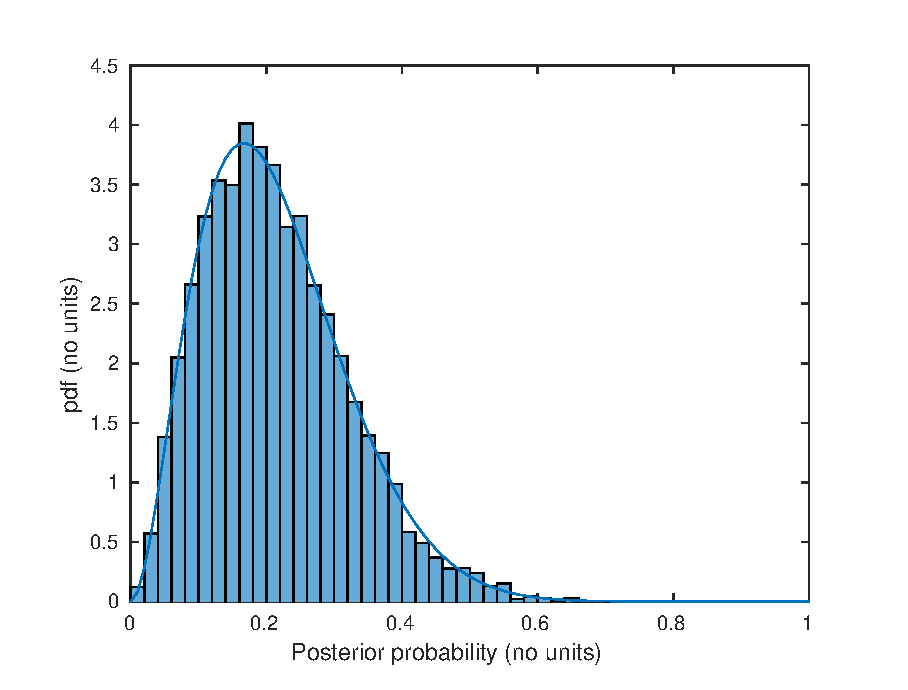
\includegraphics[width=0.5\textwidth]{binomial_ABC0528.eps}
\caption{Histogram of 10,000 samples of $\textup{Beta}(3,11)$ using ABC. The curve shows the exact posterior distribution function. The $p$-value for the $\chi^2$ goodness of fit test in this example was $5\%$ to one significant figure.}
\label{binomial}
\end{figure}

\subsection{Normal-Gamma prior, Normal likelihood}

\subsubsection{Method}
Suppose the parameters $\theta$ and $\tau$ have a prior distribution such that
\begin{equation}
\tau\sim\textup{Gamma}(\alpha_0,\beta_0)
\end{equation}
and
\begin{equation}
\mu|\tau\sim\textup{N}\left(\mu_0,1/(\nu_0\tau)\right) \ .
\end{equation}
In other words, the joint prior distribution is such that
\begin{equation}
\mu,\tau\sim\textup{NGamma}(\mu_0,\nu_0,\alpha_0,\beta_0) \ .
\end{equation}
Let a random variable $X$ given the prior be distributed such that
\begin{equation}
X|\mu,\tau\sim\textup{N}(\mu,1/\tau) \ .
\end{equation}

After observing $n$ samples of $X$, labelled $x_1,x_2,\dotdotdot ,x_n$, the joint posterior distribution is given as
\begin{equation}
(\mu,\tau|X=\{x_1,\dotdotdot ,x_n\})\sim\textup{NGamma}
\left(
	\mu_1,
	\nu_1,
	\alpha_1,
	\beta_1
\right) \ .
\end{equation}
where the posterior parameters are
\begin{align}
\mu_1 &= \dfrac{n\bar{x}+\nu_0\mu_0}{n+\nu_0} \\
\nu_1 &= n+\nu_0 \\
\alpha_1 &= \dfrac{n}{2}+\alpha_0 \\
\beta_1 &= \beta_0+\dfrac{S_{xx}}{2}+\dfrac{n\nu_0(\bar{x}-\mu_0)^2}{2(n+\nu_0)} \ ,
\end{align}
$S_{xx}$ is the sum of squared difference from the sample mean and $\bar{x}$ is the sample mean.

The marginal posterior distribution is given as
\begin{equation}
(\mu|X=\{x_1,\dotdotdot ,x_n\}) = \sqrt{\dfrac{\beta_1}{\alpha_1\nu_1}} T_{2\alpha_1}
+ \mu_1
\end{equation}
and
\begin{equation}
(\tau|X=\{x_1,\dotdotdot ,x_n\}) \sim \textup{Gamma}\left(
\alpha_1,\beta_1
\right)
\end{equation}
where $T_{2\alpha}\sim t_{2\alpha}$.

ABC can be used to sample the posterior distribution but only approximately due to the arbitrary choice of comparing two samples of continuous random variables. Here, the observed and simulated samples from ABC were compared by means of hypothesis testing on the sample mean and sample standard deviation. That is, the posterior accept/reject sampling scheme is as followed:
\begin{itemize}
	\item Sample $\tau\sim\textup{Gamma}(\alpha_0,\beta_0)$
	\item Sample $\mu|\tau\sim\textup{N}\left(\mu_0,1/(\nu_0\tau)\right)$
	\item Sample $n$ times $Y|\mu,\tau\sim\textup{N}(\mu,1/\tau)$
	\item Conduct two tailed hypothesis tests, at some confidence level, on
	\begin{equation}
	\dfrac{\sqrt{n}\left(\bar{X}-\bar{Y}\right)}{\sqrt{S_X^2+S_Y^2}}\sim\textup{N}(0,1)
	\end{equation}
	\begin{equation}
	\dfrac{S_X^2}{S_Y^2}\sim F_{n-1,n-1}
	\end{equation}
	\item Accept $\mu,\tau$ if both null hypothesis are accepted, reject otherwise
\end{itemize}
where $\bar{X}$ and $S_X^2$ are the sample mean and sample variance of the observed $X$ respectively. Similarly $\bar{Y}$ and $S_Y^2$ are the sample mean and sample variance of the simulated $Y$.

\subsubsection{Results}
The prior parameters were set to be $\mu_0=1,\nu_0=2,\alpha_0=2,\beta_0=1$. Samples of $X$ were observed by simulating $n=10$ samples from the standard Normal distribution.

1000 posterior samples were drawn using ABC with different confidence levels for the hypothesis tests. Figure \ref{surf} shows the joint histogram of the posterior samples, using a confidence level of $10\%$, compared with the true posterior distribution. By inspection, it appeared that samples from ABC is a good approximation to the posterior distribution.

The $\chi^2$ goodness of fit test was conducted on the marginal samples of the posterior distribution, as shown in Figures \ref{mean} and \ref{precision}. The $p$ values for the goodness of fit test were obtained 50 times using different observations of $X$ for different confidence levels as shown in Figures \ref{pvalue_mean} and \ref{pvalue_precision}. From the figures, there is a general trend that the $p$ values increases for smaller confidence levels as expected. However the $p$ values for confidence levels $10\%$ and $20\%$ were very similar, thus there was not much improvement in the goodness of fit test when decreasing the confidence level to $10\%.$

Figure \ref{rejections} shows the number of rejections per accepted sample when using ABC. As expected, the number of rejections increased for smaller confidence levels. However the number of rejections increased, from $(80\pm80)$ to $(1000\pm1000)$, when decreasing the confidence level from $20\%$ to $10\%$. This is an increase in the order of $10^2$.

In conclusion, a confidence level of $20\%$ is good enough for ABC to approximately sample the posterior distribution. While a confidence level of $10\%$ should give a more accurate result, it suffers from very high rejection rates.

\begin{figure}
\centering
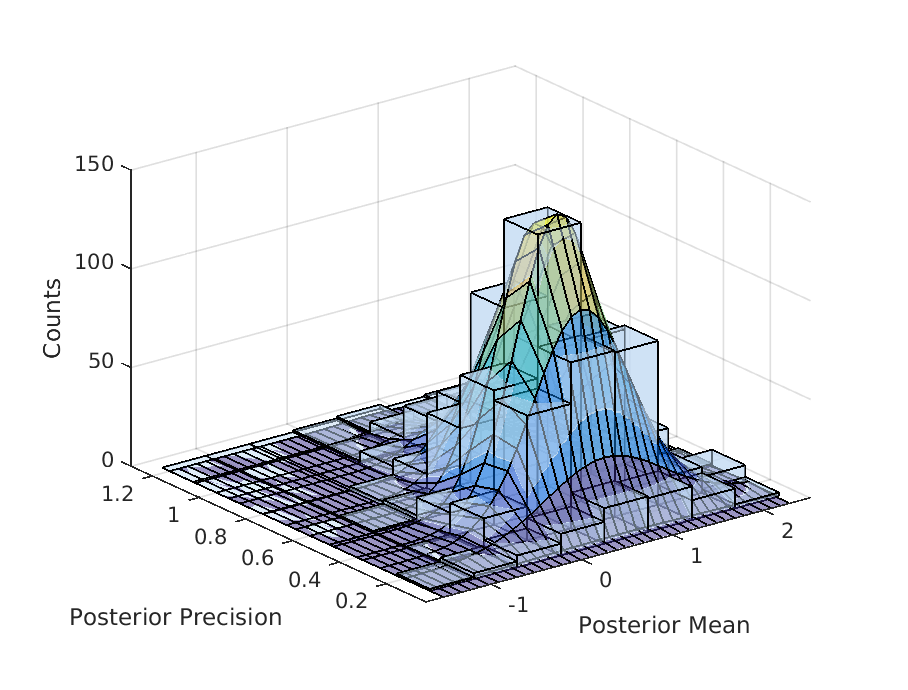
\includegraphics[width=0.5\textwidth]{surf.eps}
\caption{Joint histogram of 1000 samples of the posterior distribution using ABC compared with the true joint posterior distribution, shown as a surface plot. The confidence level was set at $10\%$ for the ABC accept/reject sampling scheme.}
\label{surf}
\end{figure}

% \begin{figure}
% 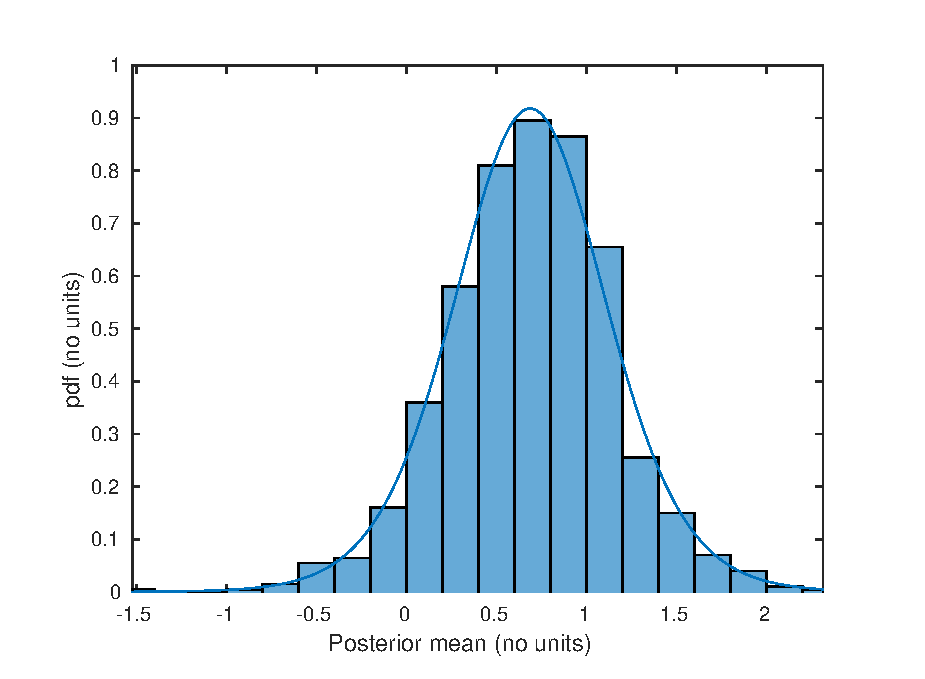
\includegraphics[width=0.5\textwidth]{mean.eps}
% \caption{Marginal histogram of 1000 samples of the posterior mean, using ABC, compared with the true marginal posterior distribution. The confidence level was set at $10\%$ for the ABC accept/reject sampling scheme. In this example, the $p$ value for the $\chi^2$ goodness of fit test was $60\%$ to one significant figure.}
% \label{mean}
% \end{figure}

% \begin{figure}
% 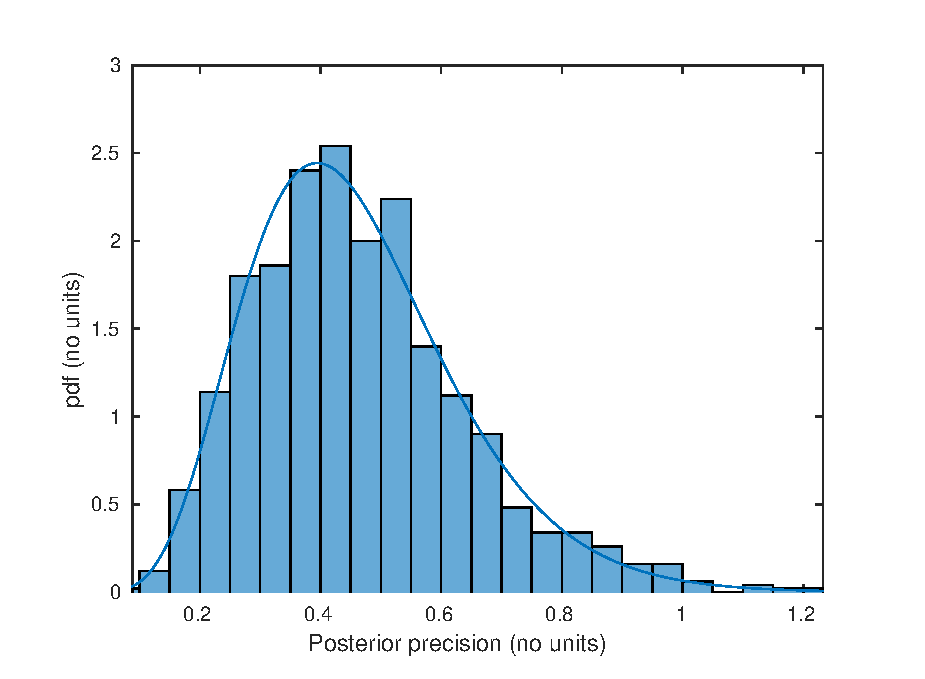
\includegraphics[width=0.5\textwidth]{precision.eps}
% \caption{Marginal histogram of 1000 samples of the posterior precision, using ABC, compared with the true marginal posterior distribution. The confidence level was set at $10\%$ for the ABC accept/reject sampling scheme. In this example, the $p$ value for the $\chi^2$ goodness of fit test was $30\%$ to one significant figure.}
% \label{precision}
% \end{figure}

\begin{figure}[htb]
\centering

\begin{subfigure}[b]{0.45\textwidth}
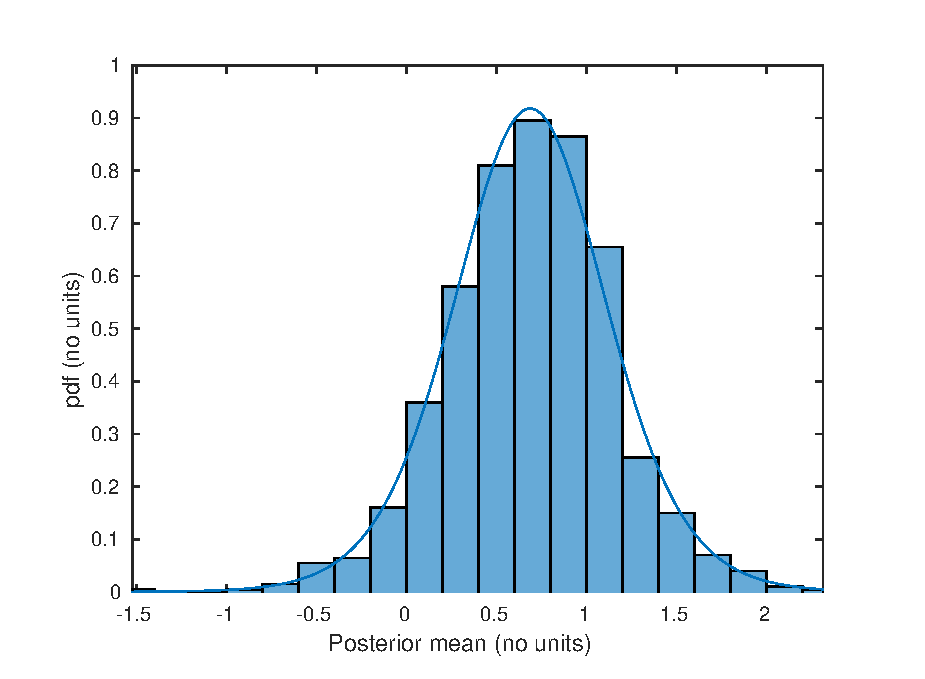
\includegraphics[width=\textwidth]{mean.eps}
\caption{Posterior mean}
\label{mean}
\end{subfigure}
\begin{subfigure}[b]{0.45\textwidth}
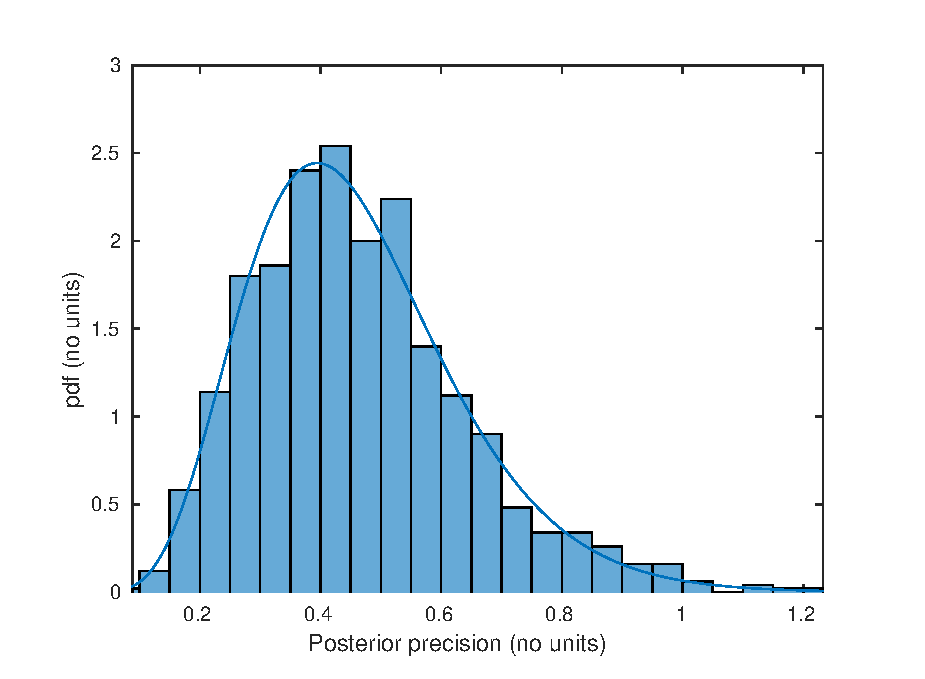
\includegraphics[width=\textwidth]{precision.eps}
\caption{Posterior precision}
\label{precision}
\end{subfigure}

\caption{Marginal histogram of 1000 samples of the posterior mean \emph{(left)} and precision \emph{(right)}, using ABC, compared with the true marginal posterior distribution. The confidence level was set at $10\%$ for the ABC accept/reject sampling scheme. In this example, the $p$ value for the $\chi^2$ goodness of fit test was $60\%$ for the mean and $30\%$ for the precision, to one significant figure .}
\label{fig:marginal}
\end{figure}


\begin{figure}[htb]
\centering

\begin{subfigure}[b]{0.45\textwidth}
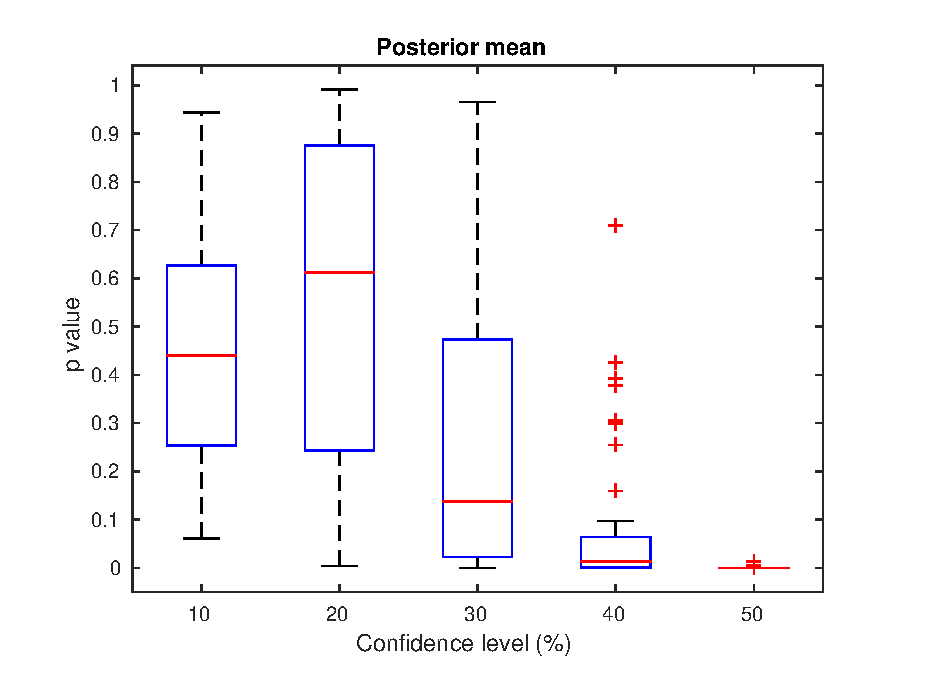
\includegraphics[width=\textwidth]{pvalue_mean.eps}
\caption{Posterior mean}
\label{pvalue_mean}
\end{subfigure}
\begin{subfigure}[b]{0.45\textwidth}
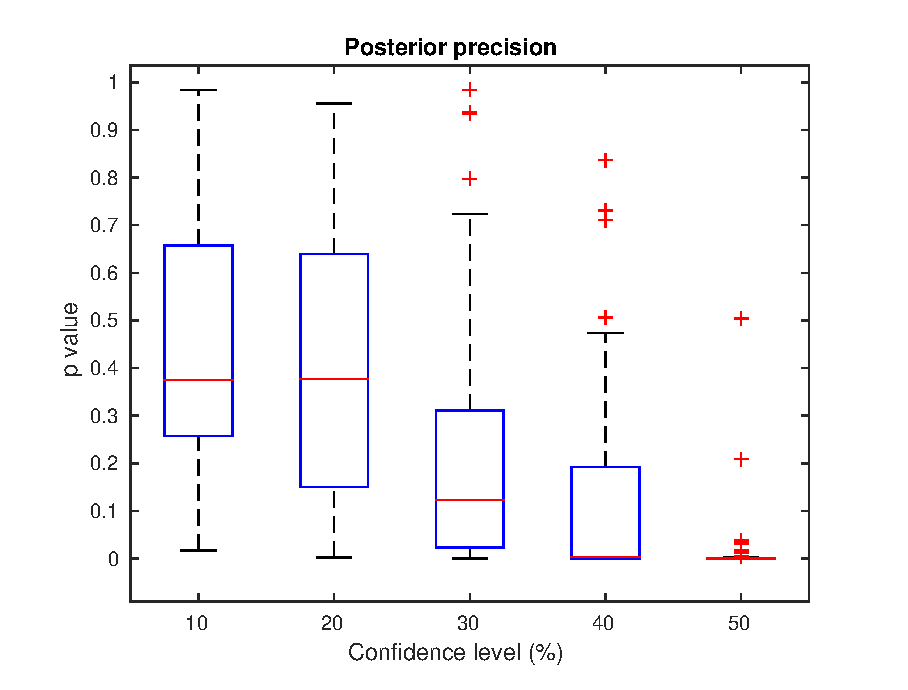
\includegraphics[width=\textwidth]{pvalue_precision.eps}
\caption{Posterior precision}
\label{pvalue_precision}
\end{subfigure}

\caption{$p$ values for the $\chi^2$ goodness of fit test on the marginal samples of the posterior mean \emph{(left)} and precision \emph{(right)}. For each confidence level, fifty $p$ values were obtained by repeating the test using different observations of the random variable $X$.}
\end{figure}

\begin{figure}[h]
\centering
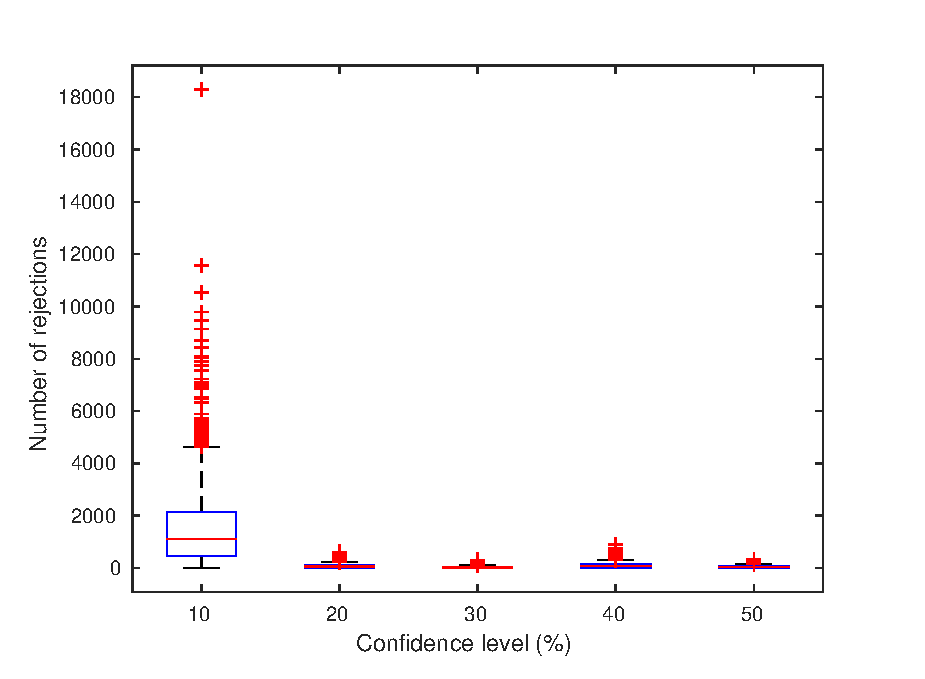
\includegraphics[width=0.5\textwidth]{rejections.eps}
\caption{The number of rejected samples per accepted sample using ABC.}
\label{rejections}
\end{figure}








\subsection{The g-and-k distribution}
We consider an implementation of ABC on data generated from the g-and-k distribution. This distribution is a flexibly shaped distribution used to model non-standard data via a small number of parameters. The distribution is defined by its inverse:

\begin{equation}
F^{-1}(x, A, B, c, g, k) = A + B\left(1 + c\frac{1-exp(-gz(x)}{1+exp(-gz(x)}\right)(1+z(x)^2)^kz(x)
\end{equation}

with parameters:
\begin{itemize}
\item A - a location parameter
\item B - a scale parameter restricted to be $>0$
\item g - controls the skewness of the data
\item k - controls the kurtosis of the data and is restricted to be $> - 0.5$
\item c - is assumed known throughout and set as 0.8
\item $z(x)$ - is the $x^{th}$ standard normal quantile
\end{itemize}

The likelihood can be calculated but it can be costly to do so. The distribution can be easily simulated from via the inversion method making it ideal for ABC. However, a suitable choice of summary statistics is not immediately obvious, as such we turn to semi-automatic ABC.

Following from the example in \cite{Fearnhead2012} we simulate an 'observed' dataset containing $10^4$ observations under the parameters, $\theta_0 = (A, B, g, k, c) = (3, 1, 2, 0.5, 0.8)$. The parameter $c$ is assumed known throughout, so we have the unknown $\theta = (A, B, g, k)$. We assume a flat prior $\theta = [0, 10]^4$.

\cite{allingham2009}, in analysing these data used the full order statistics as the summary statistics. Following from \cite{Fearnhead2012} we consider a number of order statistics for $m = 60, \ldots, 140)$, and transformations of these $f(x) = (x^1, \ldots, x^l)$ as these correspond to the position, scale, skewness, and kurtosis of the data, which should give better information regarding the parameters $g$ and $k$.


\begin{table}[h]
\centering
\label{tab:bic}
  $\begin{tabu}{| l | r | r | r | r | r|}
  \hline			
    & A & B & g & k & mean \\
    \hline
  m = 60, l = 1 	& -477,275.1 & -144,985.4	 & 359,180.7	 & 359,142.5  & 24,015.675 \\
  m = 60, l = 2  	& -477,238.5 & -146,515.7	 & 346,921.0 	 & 314,714.5 & 9,470.325  \\
  m = 60, l = 3 	& -477,115.1 & -147,346.7	 & 339,500.3  	 & 289,321.1 & 1,089.9 \\
  m = 60, l = 4 	& -476,789.4 & -147,788.8	 & 333,963.4  	 & 267,438.7 & -5,794.025 \\
  \hline
  m = 100, l = 1 	& -475,500.9 & -142,653.4  & 359,574.0 	 & 359,592.1 & 25,252.95 \\
  m = 100, l = 2  	& -475,192.0 & -144,027.1	 & 347,352.0 	 & 315,207.7 & 10,835.15\\
  m = 100, l = 3 	& -474,537.7 & -144,383.6	 & 340,605.3 	 & 290,100.3 & 2,946.075 \\
  m = 100, l = 4 	& -473,801.6 & -144,328.4	 & 335,512.2 	 & 268,829.3 & -3,447.125 \\
  \hline
  m = 140, l = 1 	& -476,547.0 & -144,126.4  & 360,009.4		 & 359,916.1 & 24,813.025  \\
  m = 140, l = 2  	& -475,741.5 & -144,858.0  & 348,367.8   	 & 316,093.5 & 10,965.45\\
  m = 140, l = 3 	& -474,795.7 & -144,865.4  & 341,789.4 	 & 291,313.5 & 3,360.45   \\
  m = 140, l = 4 	& -473,678.3  & -144,479.1   & 337,162.2    & 270,057.9 & -2,734.325  \\
  \hline 
  \end{tabu} $
    \caption{The BIC resulting from inferring the parameter values from the order statistics for a variety of number of order statistics ($m$), and powers of these ($l$)}
\end{table}

We consider the best model for inferring the parameter values as that with the lowest average BIC value across parameters. Similar to \cite{Fearnhead2012} we find that the BIC is minimised as we increase the powers of our summary statistics to be used in the ABC algorithm. Figure 6 shows the additional inferential power of  the higher powers, particularly in relation to parameters g and k. However, where they found the BIC minimised at 100 order statistics, we found it minimised at a lower value of 60.

\begin{figure}[h]
\label{fig:powers}
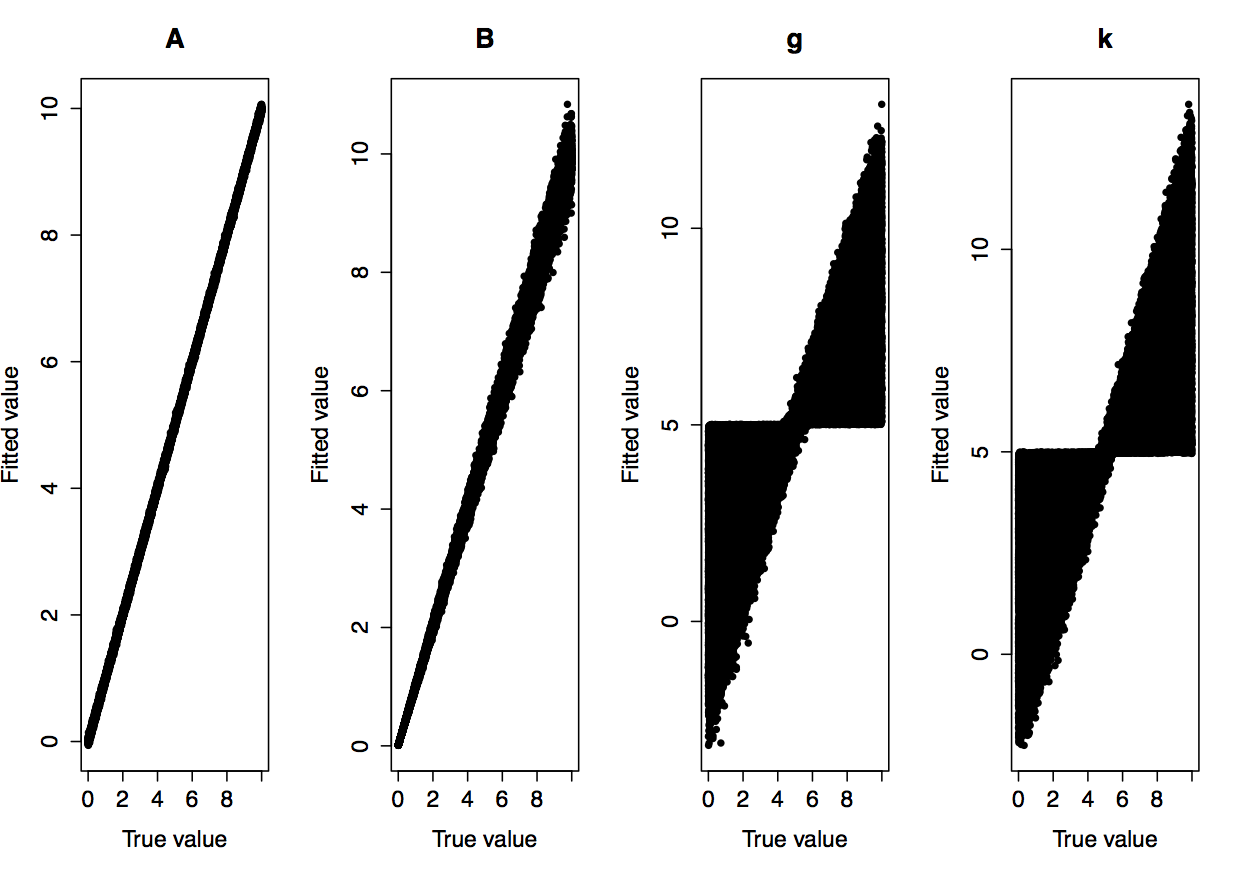
\includegraphics[width = \linewidth]{firstorder.pdf}
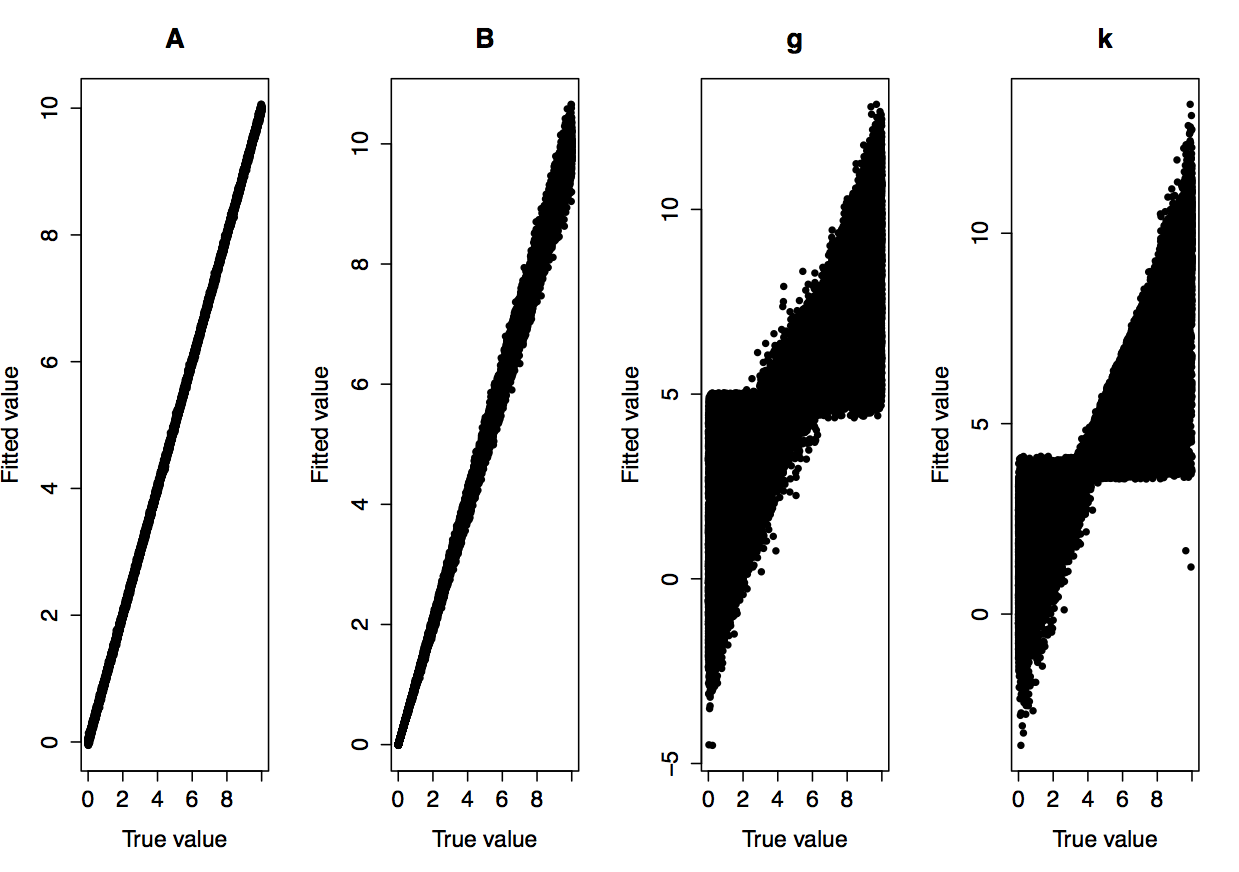
\includegraphics[width = \linewidth]{fourthorder.pdf}
\caption{Fitted parameter values vs actual parameter value from the summary statistics selection stage of the semi-auto ABC algorithm with 1 power included (top) and 4 powers included (bottom).}
\end{figure}



Given the summary statistics selected above, we proceed to perform the ABC analysis, using the \texttt{abc} and \texttt{abctools} packages in R.
We performed cross-validation to select $\epsilon$, the tolerance level. We used the methods of rejection sampling and local linear regression to perform the ABC. Local linear regression produced a posterior closer to the true value than rejection sampling. We present the posterior for the parameters calculated from  ABC using local linear regression in Figure \ref{fig:HIST}. 

We also implemented semi-automatic ABC on these data. Results are shown in Figures \ref{fig:HIST_SA} to \ref{fig:CONT_GK}. It can be seen that the posterior distributions from the semi-automatic ABC appears tighter around the true parameter values than in the case of the ABC approach.





\begin{figure}
\label{fig:HIST}
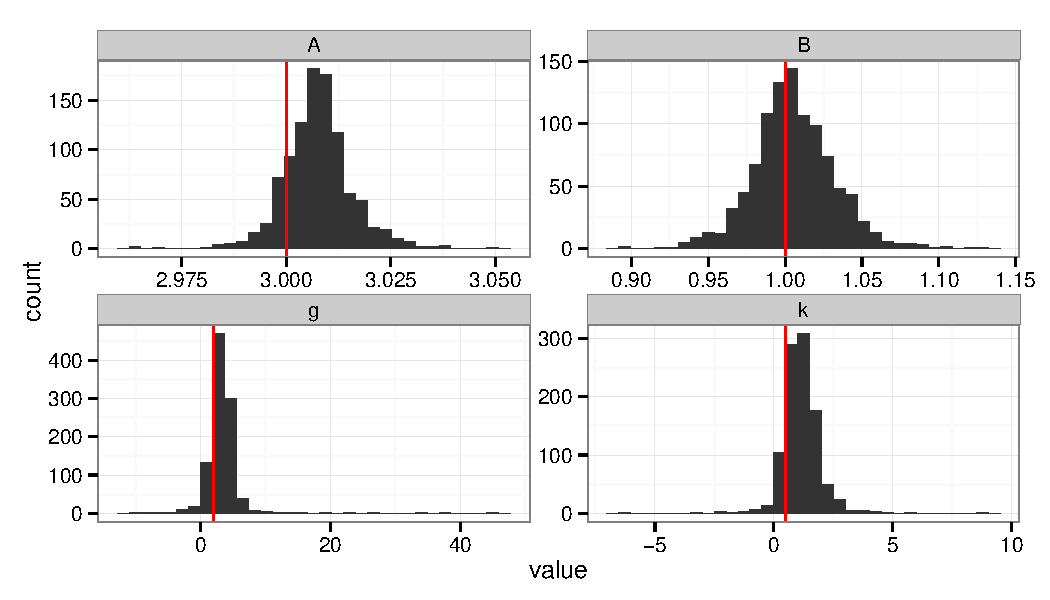
\includegraphics[width = \linewidth]{GK_REG_M_HIST.pdf}
\caption{Histogram of posterior parameter estimates with true values indicated in red under the ABC with local linear regression}
\end{figure}

\begin{figure}
\label{fig:HIST_SA}
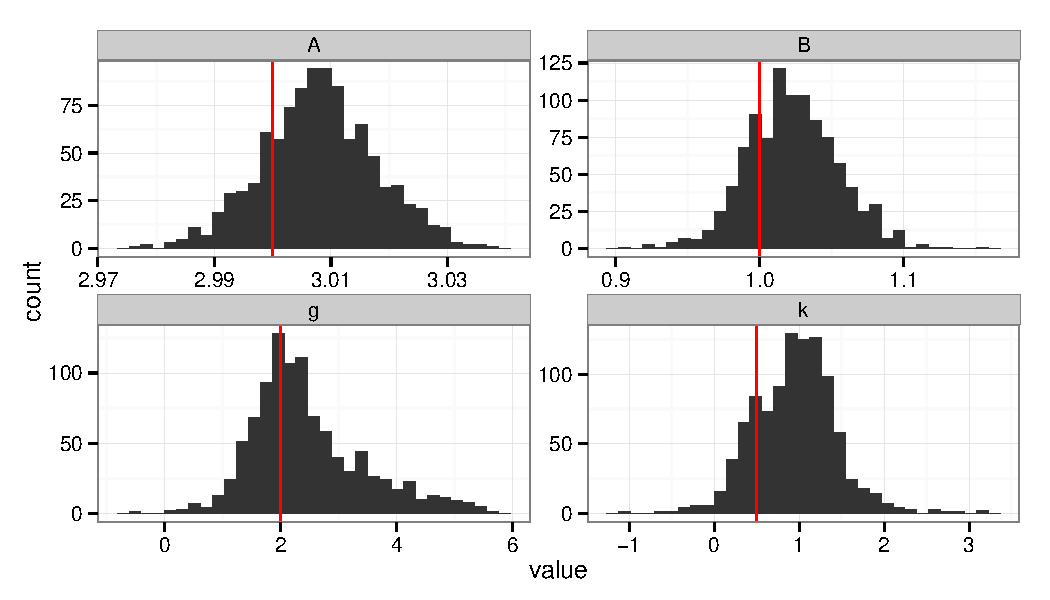
\includegraphics[width = \linewidth]{GK_REG_M_HIST_SA.pdf}
\caption{Histogram of posterior parameter estimates with true values indicated in red under the semi-automatic ABC with local linear regression}
\end{figure}

\begin{figure}
\label{fig:CONT_AB}
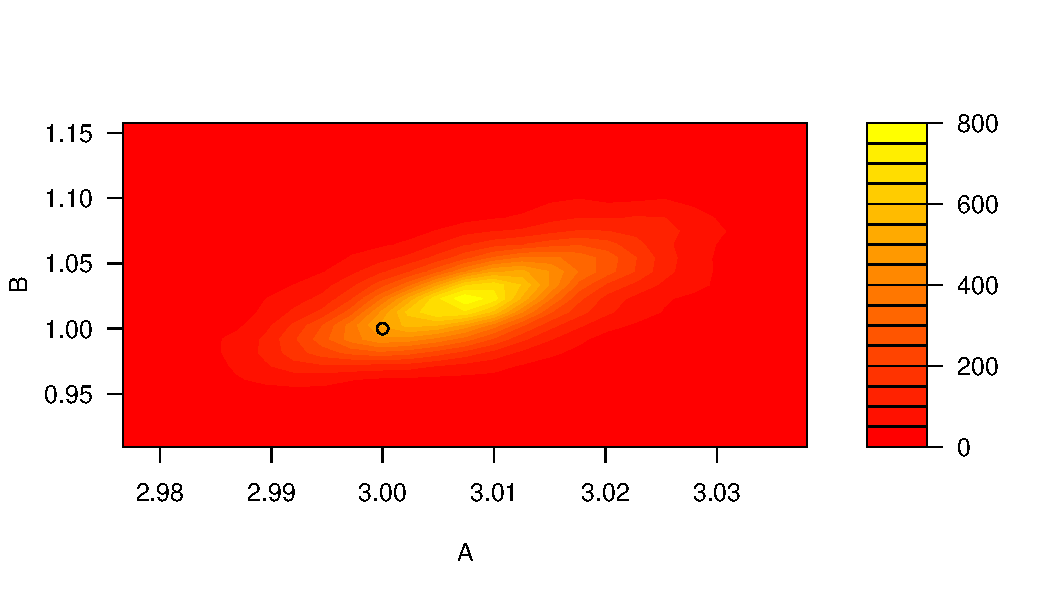
\includegraphics[width = \linewidth]{GK_REG_M_CONT_AB_SA.pdf}
\caption{Contour plot of posterior parameter estimates for A and B with true values indicated in black under the semi-automatic ABC with local linear regression}
\end{figure}

\begin{figure}
\label{fig:CONT_GK}
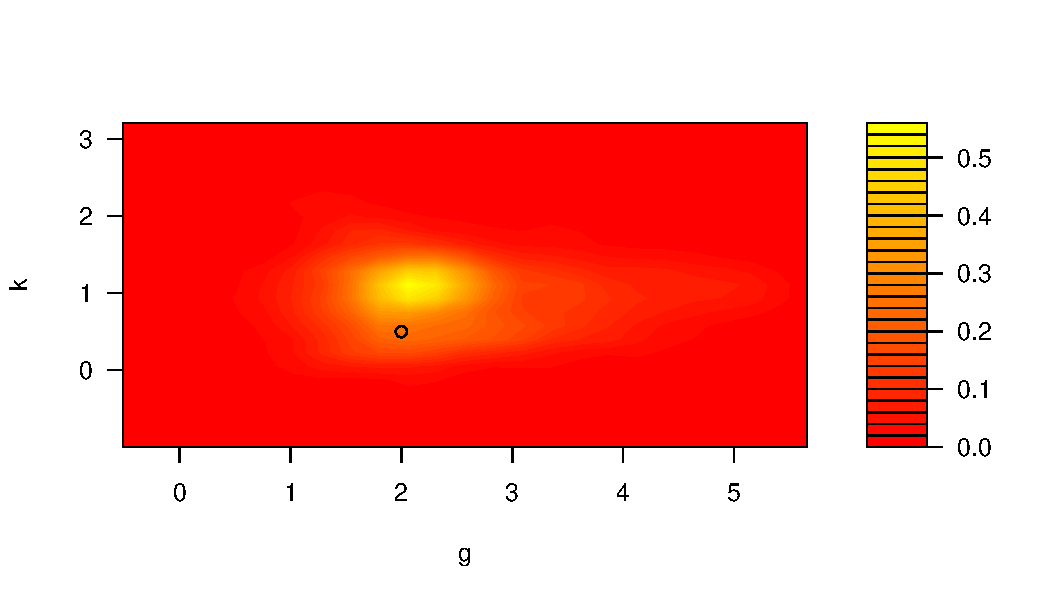
\includegraphics[width = \linewidth]{GK_REG_M_CONT_GK_SA.pdf}
\caption{Contour plot of posterior parameter estimates for g and k with true values indicated in black under the semi-automatic ABC with local linear regression}
\end{figure}


\section{Conclusion}
In this report, we found that in ABC can approximate the posterior distribution well but can suffer from high rejection rates. A good confidence level, or threshold, is one which is small enough that samples, drawn from ABC, approximates the posterior distribution well but big enough the rejection rate is feasible.

We have only just scratched the surface in terms of literature available for extensions to the basic ABC methods. Further work would include exploring sequential implementations of ABC which are known to be more efficient although attention still needs to be given to tuning the parameters.




\bibliography{ABC}
\end{document}

\begin{figure}[h] 
\centering
\includegraphics[width=0.6\textwidth]{graph_nd.pdf}
\caption{The Chen-Stein bounds on the distance between $\mathbb{P}(W=0)$ and $\mathbb{P}(Z=0)$ as $n$ increases, keeping the ratio $\frac{n^k}{d^{1-k}}$ constant at 1.45.}
\label{fig:graph_nd}
\end{figure}